% "Станет проще"

\documentclass[12pt]{article}

% report, book

%  Русский язык

\usepackage[T2A]{fontenc}
\usepackage[utf8]{inputenc}
\usepackage[english,russian]{babel}

\usepackage{geometry}
\geometry{a4paper}

\usepackage{amsmath,amsfonts,amssymb,amsthm,mathtools} 

\usepackage{graphicx}


\usepackage{wasysym}

\usepackage{geometry} 
\geometry{a4paper,top=2cm,bottom=3cm,left=2cm}



\begin{document} % начало документа

\newpage

\section{Система Лоренца}

Об объекте можно говорить, как о динамической системе, если можно указать такой набор величин, называемых динамическими переменными и характеризующих состояние системы, что их значения в любой последующий момент времени получаются из исходного набора по определенному правилу.

Хоть и по определению динамической системы всегда можно однозначно предсказать конечное состояние по исходному, но в ней все равно может возникать хаос. В хаотическом режиме любая неточность в задании начального состояния нарастает во времени, так что предсказуемость становится недостижимой на достаточно больших интервалах времени. Такого рода режимы характеризуются нерегулярным, хаотическим изменением динамических переменных во времени.

Аттрактор Лоренца ― \textbf{компактное инвариантное множество} L в трехмерном фазовом пространстве гладкого потока. Система уравнений имеет вид
$$\begin{cases}	
	\dot{x} = \sigma (y-x) \\
	\dot{y} = x(\rho-z)-y \\
	\dot{z} = xy-bz
\end{cases}$$

Эта модель была впервые описана в 1963 году Эдвардом Лоренцом в статье "Детерминированное непериодическое течение". Лоренц получил эту модель как линейную аппроксимацию гидродинамической системы уравнений для задачи о конвекции морской воды в плоском слое; значения параметров и начальные условия были выбраны таким образом: $\sigma = 10$, $\rho = 28$, $b = \frac{8}{3}$; $x(0) = 1$, $y(0) = 0$, $z(0) = 0$.

Модель Лоренца является реальным физическим примером динамических систем с хаотическим поведением, в отличие от различных искусственно сконструированных отображений.

\section{Конвекция в замкнутой петле}

Трубка, замкнутая в кольцо, наполнена почти несжимаемой жидкостью. Она подогревается снизу и охлаждается сверху, и при достаточно сильном нагреве возможно возникновение конвекционного течения.

\begin{figure}[h]
	\centering
 	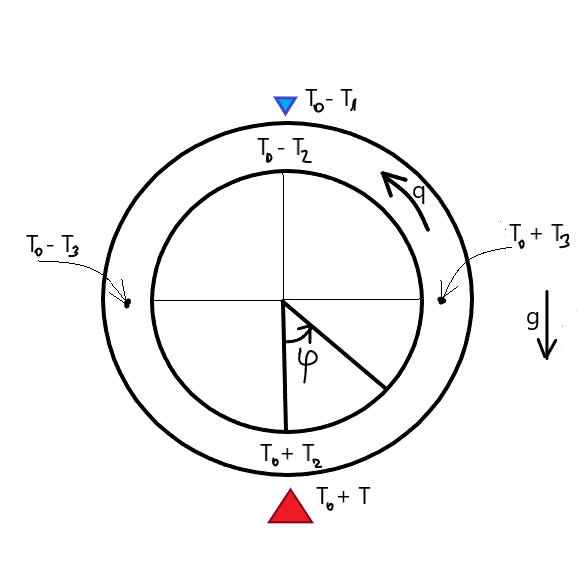
\includegraphics[scale=0.5]{Lorenz.png}
 	\caption{Кольцо с подогревом.}
  	\label{fig:boat1}
\end{figure}

Заметим, что раз жидкость почти несжимаемая, то ее скорость во всех точках трубки постоянна, она не зависит от $\phi$. Обозначим скорость за $X$.

Температура жидкости в трубке будет зависить от угла $\phi$, который отсчитывается от направленного вниз радиуса до точки против часовой стрелки. $T = T(\phi) -$ периодическая функция (период равен $2\pi$) $\Rightarrow$ ее можно разложить в ряд Фурье.

При разложении основную амплитуду задают первые слагаемые, поэтому рассмотрим только первую гармонику. Уравнение будет иметь вид $T = T_0 \cdot (1+Ysin\phi + Zcos\phi)$. Исследуем коэффициенты при $sin\phi$ и $cos\phi$.

Отклонение температуры от радиуса, направленного к нагревателю зависит от $cos \phi$, значит $Z$ характеризует отклонение температуры от среднего значения в точке нагрева (нижней точки трубки). Отклонение от крайней правой точки (на 3 часа, то есть $\phi = \frac{\pi}{2}$) зависит от $sin\phi$, и $Y$ его характеризует.

Рассмотрим, что вызывает изменение скорости жидкости. Во-первых, действует сила Архимеда, она пропорциональна $Y$, так как в $\phi=\frac{\pi}{2}$ она направлена вверх. Во-вторых, действует сила вязкости, которая пропорциональна скорости, следовательно, пропорциональна $X$. Тогда

\begin{equation}
	\dot{X} = cY-\beta X
\end{equation}

Пусть течение происходит с постоянной скоростью, то есть угол изменяется на $Xt$. Тогда

\begin{equation}
	T=f(\phi-Xt)=T_0(1+Ysin(\phi-Xt)+Zcos(\phi-Xt))
\end{equation}

Пусть $\phi'=\phi-Xt$, тогда

\begin{equation}
	\dot{T}=T_0(Y(-X)cos\phi'-Z(-X)sin\phi')=T_0(ZXsin\phi'-YXcos\phi')
\end{equation}

Вспомним, что за отклонение температуры от нижней точки отвечал $cos\phi \Longrightarrow$ перенос температуры потоком жидкости для $Z$ учитывается членом $-YX$. Аналогично, для $Y$ будет $ZX$.

В точке $Z$ происходит постоянный подогрев, поэтому в уравнении будем его учитывать, добавив константу $A$. 

В системе стремится установиться термодинамическое равновесие, следовательно, надо учитывать в уравнениях для $Y$ и $Z$ релаксацию, это будут члены $-DY$ и $-DZ$ соотвественно, где $D -$ постоянная величина.

Таким образом

$$\begin{cases}
	\dot{X} = cY-\beta X \\
	\dot{Y} = XZ-DY \\
	\dot{Z} = A-XY-DZ
\end{cases}$$

Заменим переменные: $X=Dx, Y=\frac{\beta Dy}{c}, Z=-\frac{\beta Dz}{c}$, тогда

$$\begin{cases}	
	\dot{x} = \sigma (y-x) \\
	\dot{y} = x(\rho-z)-y \\
	\dot{z} = xy-bz
\end{cases}$$

где $\sigma = \frac{\beta}{D}, \rho=\frac{cA}{\beta D^2}, b=1$.

Таким образом, были получены уравнения Лоренца.

\section{Другие области применения}

Модель Лоренца применима в других физических процессах:
\begin{itemize}
	\item Конвекция в плоском слое
	\item Вращение водяного колеса (колесо, на ободе которого укреплены корзины с отверстиями в дне; сверху на колесо симметрично относительно оси вращения льётся сплошной поток воды)
	\item Одномодовый лазер
	\item Диссипативный осциллятор с инерционным возбуждением
\end{itemize}

При этом в других моделях переменные и параметры будут иметь другой смысл. Так для конвекции в плоском слое $x$ отвечает за скорость вращения водяных валов, $y$ и $z$ -- за распределение температуры по горизонтали и вертикали, $\rho$ -- нормированное число Рэлея, $\sigma$ -- число Прандтля (отношение коэффициента кинематической вязкости к коэффициенту температуропроводности), $b$ содержит информацию о геометрии конвективной ячейки. 

Вращение водяного колеса похоже по поведению на конвецкцию в замкнутой петле с точностью до переворота "вверх ногами", поэтому описывается аналогичными уравнениями с заменой температуры на плотность распределения массы воды в корзинах по ободу.

Для одномодового лазера $x$ -- амплитуда волн в резонаторе лазера, $y$ -- поляризация, $z$ -- инверсия населённостей энергетических уровней, $b$ и $\sigma$ -- отношения коэффициентов релаксации инверсии и поля к коэффициенту релаксации поляризации, $\rho$ -- интенсивность накачки.


\end{document} % конец документа